\chapter{블랙홀 만들기와 지평선 근처의 수수께끼}

\lectureoverview{평탄 시공간의 인과도, 슈바르츠실트 도표, 구형 껍질에 대한 버코프 정리, 이렇게 세 가지를 이용해 블랙홀을 만들어 보겠습니다. 이 구성은 사건의 지평선이 전역적인 경계이며, 국소적으로는 여전히 평탄한 영역에서 시작될 수 있음을 보여 줍니다. 그런 다음 인과 기하학에서 엔트로피와 호킹 온도로 넘어갑니다. 지평선 가까이에 둔 온도계는 한없이 뜨거워지지만, 자유 낙하하는 관측자는 국소적으로 아무런 재앙도 없으리라 예상합니다. 마지막 논의에서는 외부 관측자가 자신이 감지하려는 교란을 일으키지 않고 실제로 무엇을 알아낼 수 있는지 묻습니다.}

\section{빈 공간의 온도를 지닌 블랙홀}

과제로 블랙홀을 만들어 수업에 가져와 발표하기로 했습니다. 보여 줄 블랙홀을 가진 사람은 없었지만, Wolfram에서 찾은 계산을 바탕으로 좀 더 부담 없는 도입 문제를 풀어 보았습니다. 호킹 온도가 우주 마이크로파 배경의 \(3\,\mathrm{K}\) 온도에 가까운 블랙홀의 반지름과 질량은 얼마일까요?

\begin{classroomqa}
\audiencequestion{웹사이트에서 계산한 것은 무엇이었나요?\lecturetimestamp{00:00:39}}
\lecturerresponse{온도가 대략 \(3\,\mathrm{K}\)인 블랙홀의 반지름입니다. 여기서 중요한 것은 정밀한 계산이 아니라 물리적 규모를 추정하는 것입니다.}
\end{classroomqa}

그런 블랙홀은 잠시 주변과 같은 온도를 갖겠지만, 그 평형은 불안정합니다. 슈바르츠실트 블랙홀은 열용량이 음수입니다. 열저장고보다 조금 더 뜨거워지면 복사를 방출하고 질량을 잃어 더욱 뜨거워집니다. 조금 더 차가워지면 복사 에너지를 흡수하고 질량이 늘어 더욱 차가워집니다.\editorialnote{일부러 느슨하게 표현한 수업 내용의 배경에는 바로 이 안정성 논증이 있습니다. 정준 열저장고는 고립된 슈바르츠실트 블랙홀에 안정적인 평형을 제공할 수 없습니다.}

추정은 \(3\,\mathrm{K}\) 복사의 대표 파장에서 시작합니다.

\begin{classroomqa}
\audiencequestion{약 3켈빈의 복사에는 어떤 파장이 해당하나요?\lecturetimestamp{00:02:03}}
\lecturerresponse{강의실에서는 센티미터, \(21\) 센티미터, 심지어 \(10\) 미터까지 여러 규모가 거론되다가 마이크로파 영역으로 정리되었습니다. 논의에 유용한 대략적인 규모의 답은 약 한 센티미터였습니다. 전자레인지와 빵 보관함을 두고 농담하기에 충분히 작은 크기였지요.}
\end{classroomqa}

전형적인 호킹 양자의 파장은 수치 계수를 제외하면 슈바르츠실트 반지름과 비슷합니다:
\begin{equation}
\lambda_{\mathrm{H}}\sim R_s,
\qquad
R_s=\frac{2GM}{c^2}.
\label{eq:l05-scale}
\end{equation}
수업에서 사용한 값 \(\lambda_{\mathrm H}\sim1\,\mathrm{cm}\)을 대입하면 \(R_s\sim1\,\mathrm{cm}\)을 얻습니다. 태양 질량 블랙홀의 반지름은 수 킬로미터이고 \(R_s\)는 \(M\)에 비례하므로, 이에 해당하는 질량은 대략
\begin{equation}
M\sim10^{-5}M_\odot,
\label{eq:l05-rough-mass}
\end{equation}
행성 규모입니다. 그래서 강의에서는 지구와 비슷한 규모의 추정값이 나옵니다.

\begin{classroomqa}
\audiencequestion{Wolfram의 수치 결과와 일치하나요?\lecturetimestamp{00:05:53}}
\lecturerresponse{보고된 결과는 달의 질량에 더 가까웠습니다. 대략적인 추정과 비교하면 작아 보이지만, 어느 쪽이든 요점은 같습니다. 주머니에 넣고 다닐 수 있는 물체가 아니라는 것입니다.}
\end{classroomqa}

상수들을 포함하면 차이가 설명됩니다. 다음 식에서
\begin{equation}
T_H=\frac{\hbar c}{4\pi k_B R_s},
\end{equation}
\(T_H=3\,\mathrm{K}\)일 때
\begin{equation}
R_s\simeq6.1\times10^{-5}\,\mathrm{m},
\qquad
M\simeq4.1\times10^{22}\,\mathrm{kg}.
\label{eq:l05-three-kelvin}
\end{equation}을 얻습니다.
이는 지구 질량이 아니라 달 질량에 해당합니다. 마이크로파 파장, 계수 \(4\pi\), 그리고 어떤 흑체 파장을 대표값으로 삼는지에 따라 간단한 추정과 수치값 사이에 차이가 생깁니다.\editorialnote{~\eqref{eq:l05-three-kelvin}식은 강의의 차원 분석 추정에서 생략한 수치 계수를 복원합니다. 수업에서 사용한 전개를 보여 주기 위해 추정 자체도 그대로 두었습니다.}

계산은 제 역할을 다했습니다. 이제 수학적으로, 그리고 상상 속에서 블랙홀을 만들어 보겠습니다. 지금 목적에 필요한 전체 장방정식은 다루기 너무 어렵습니다. 기본적인 사실은 그림으로 살펴보겠습니다.

\section{첫 번째 구성 요소: 평탄 시공간}

관측자를 중심으로 한 극좌표를 쓰고 각도 좌표는 생략합니다. 축약한 좌표는 \((t,r)\)이며, \(r\geq0\)입니다. 이 축약 도표의 한 점은 4차원 시공간의 한 점이 아닙니다. \(r=0\)인 경우를 제외하면, 점 하나가 구면 \(S^2\) 전체를 나타냅니다.

방사형 빛살은 \(45^\circ\) 방향으로 움직입니다. 안쪽으로 향하는 빛살은 원점에 도달하고, 바깥쪽으로 향하는 빛살은 다른 영방향을 따라 원점에서 멀어집니다. 무한한 반평면은 등각변환으로 유한한 펜로즈 쐐기에 압축할 수 있습니다. 변환은 유일하지 않습니다. 핵심은 무한대를 유한한 경계로 옮기고 방사형 영방향을 \(45^\circ\)로 유지하는 것입니다. 칠판에서 쓴 표현대로, 도표를 뭉개서 줄입니다.

\begin{figure}[htbp]
\centering
\includegraphics[width=0.68\textwidth]{lecture_05_figure_02.png}
\caption{콤팩트화한 방사형 민코프스키 시공간의 위쪽 절반. 수직 경계는 \(r=0\)이고, 곡선들의 모임은 콤팩트화된 무한대 쪽으로 몰립니다.}
\lectureframe{00:11:41.560}
\end{figure}

\begin{figure}[htbp]
\centering
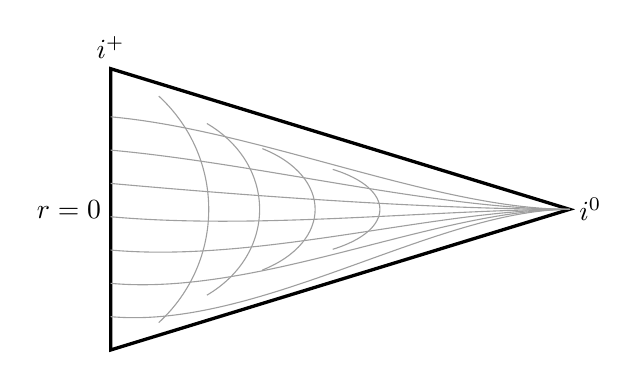
\begin{tikzpicture}[scale=0.94]
\coordinate (O) at (0,0);
\coordinate (P) at (0,3.8);
\coordinate (I) at (6.2,1.9);
\draw[very thick] (O)--(P)--(I)--cycle;
\foreach \y in {0.45,0.90,1.35,1.80,2.25,2.70,3.15} {
  \draw[gray!75] (0,\y) .. controls (2.0,\y-0.18) and (4.4,1.9) .. (I);
}
\draw[gray!75] (0.65,0.37) .. controls (1.55,1.20) and (1.55,2.60) .. (0.65,3.43);
\draw[gray!75] (1.30,0.74) .. controls (2.25,1.30) and (2.25,2.50) .. (1.30,3.06);
\draw[gray!75] (2.05,1.08) .. controls (3.00,1.46) and (3.00,2.34) .. (2.05,2.72);
\draw[gray!75] (3.00,1.36) .. controls (3.85,1.62) and (3.85,2.18) .. (3.00,2.44);
\node[left] at (0,1.9) {\(r=0\)};
\node[above] at (P) {\(i^+\)};
\node[right] at (I) {\(i^0\)};
\end{tikzpicture}
\caption{정돈된 위쪽 쐐기. 곡선들은 정성적인 상수 \(r\) 및 상수 \(t\) 곡선군이며, 정확한 좌표 격자는 아닙니다.}
\label{fig:l05-flat-wedge}
\end{figure}

고정된 \(r\)에서의 세계선은 콤팩트화 전에는 수직이지만, 휘어지며 미래 시간꼴 무한대 근처에 모입니다. 상수 \(t\) 단면도 마찬가지로 공간꼴 무한대 쪽으로 몰립니다. 이렇게 몰리는 것은 좌표 효과이지, 물질이 물리적으로 압축되는 현상이 아닙니다.

\(45^\circ\) 법칙은 방사 방향으로 진행하는 빛에 직접 적용됩니다. 각운동량이 있는 광선은 원점을 빗겨 가며, 영이 아닌 최근접 거리에 도달한 뒤 다시 바깥쪽으로 나아갈 수 있습니다. 원점에서 멀리 떨어진 곳에서는 그 투영된 운동이 거의 방사형으로 보입니다. 축약된 \((t,r)\) 궤적이 눈에 띄게 휘는 곳은 최근접 지점 부근뿐입니다. 이것으로 첫 번째 실질적 논의 부분을 마칩니다.

\section{두 번째 구성 요소: 영원한 슈바르츠실트}

최대 연장 슈바르츠실트 해에는 두 개의 외부 다이아몬드, 미래 블랙홀 영역, 과거 화이트홀 영역이 있습니다. 위아래의 물결 모양 경계는 각각 미래 특이점과 과거 특이점입니다. 붕괴로 만들어진 블랙홀을 다룰 때는 이 구조 대부분을 곧 버리겠지만, 오른쪽의 보통 외부 영역은 정확히 필요한 부분입니다.

\begin{figure}[htbp]
\centering
\includegraphics[width=0.72\textwidth]{lecture_05_figure_03.png}
\caption{오른쪽에 보통의 외부 영역과 그 안의 개략적인 좌표 격자를 표시한 영원한 슈바르츠실트 도표.}
\lectureframe{00:16:55.975}
\end{figure}

\begin{figure}[htbp]
\centering
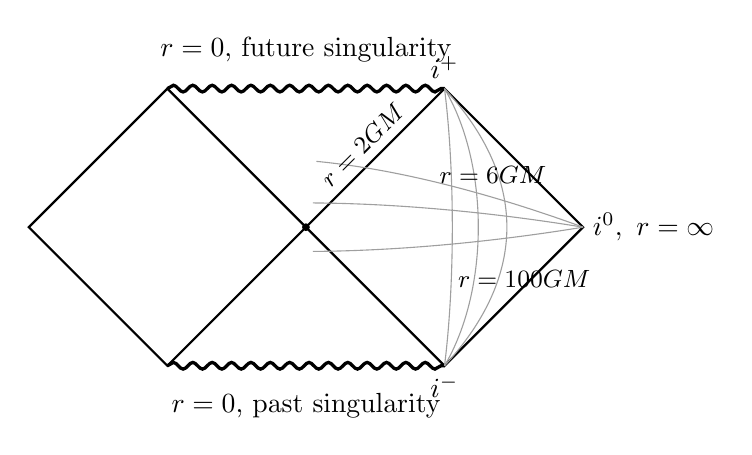
\begin{tikzpicture}[scale=0.88]
\coordinate (C) at (0,0);
\coordinate (TL) at (-2.0,2.0);
\coordinate (L) at (-4.0,0);
\coordinate (BL) at (-2.0,-2.0);
\coordinate (TR) at (2.0,2.0);
\coordinate (R) at (4.0,0);
\coordinate (BR) at (2.0,-2.0);
\draw[thick] (C)--(TL)--(L)--(BL)--(C);
\draw[thick] (C)--(TR)--(R)--(BR)--(C);
\draw[very thick,decorate,decoration={snake,amplitude=1.2pt,segment length=7pt}] (TL)--(TR);
\draw[very thick,decorate,decoration={snake,amplitude=1.2pt,segment length=7pt}] (BL)--(BR);
\draw[gray!75] (TR) .. controls (2.15,0.8) and (2.15,-0.8) .. (BR);
\draw[gray!75] (TR) .. controls (2.65,0.9) and (2.65,-0.9) .. (BR);
\draw[gray!75] (TR) .. controls (3.20,0.7) and (3.20,-0.7) .. (BR);
\draw[gray!75] (0.15,0.95) .. controls (1.5,0.82) and (2.9,0.40) .. (R);
\draw[gray!75] (0.10,0.35) .. controls (1.5,0.34) and (2.9,0.18) .. (R);
\draw[gray!75] (0.10,-0.35) .. controls (1.5,-0.34) and (2.9,-0.18) .. (R);
\fill (C) circle (1.6pt);
\node[above] at (TR) {\(i^+\)};
\node[below] at (BR) {\(i^-\)};
\node[right] at (R) {\(i^0,\ r=\infty\)};
\node[above] at (0,2.25) {\(r=0\), future singularity};
\node[below] at (0,-2.25) {\(r=0\), past singularity};
\node[rotate=45,above,font=\small] at (1.0,1.0) {\(r=2GM\)};
\node[font=\small] at (2.70,0.75) {\(r=6GM\)};
\node[font=\small] at (3.15,-0.75) {\(r=100GM\)};
\end{tikzpicture}
\caption{오른쪽 외부 영역은 큰 반지름에서 평탄 쐐기와 닮았습니다. 안쪽의 영방향 경계는 \(r=2GM\)이며 \(c=1\)일 때 그렇습니다. 다른 반지름 표시는 예시를 위한 개략값입니다.}
\label{fig:l05-eternal-schwarzschild}
\end{figure}

블랙홀에서 멀리 떨어진 외부 영역은 콤팩트화된 평탄 공간에 점점 가까워집니다. \(r=6GM\) 및 \(r=100GM\) 같은 선은 보통의 일정한 반지름 세계선의 거동에 가까워집니다. 외부 영역의 안쪽 경계는
\begin{equation}
r=2GM
\end{equation}
단위계 \(c=1\)에서 주어집니다.

중심 근처에서는 평탄 공간과의 비교가 성립하지 않습니다. 민코프스키 시공간의 방사형 빛살은 \(r=0\)에 도달한 뒤 반대쪽 물리적 방향으로 다시 나옵니다. 슈바르츠실트 영역 안의 미래지향 빛살은 튕겨 나오지 않습니다. \(r=0\)의 공간꼴 특이점에서 끝납니다. 붕괴 시공간을 구성할 때 보존해야 하는 인과 구조의 차이가 바로 이것입니다.

\section{구성 요소들을 이어 붙이게 해 주는 정리}

빠진 요소는 뉴턴 중력에서 처음 나타납니다. 구대칭 질량 분포에 대해 가우스 법칙은
\begin{equation}
\oint\mathbf g\cdot d\mathbf A=-4\pi G M_{\mathrm{enc}},
\end{equation}
을 주며, 따라서
\begin{equation}
\mathbf g(r)=-\frac{G M_{\mathrm{enc}}(r)}{r^2}\,\hat{\mathbf r}.
\label{eq:l05-shell-theorem}
\end{equation}
입니다.
반지름 \(r\)인 구 바깥의 물질은 그 구에서 알짜장을 만들지 않습니다. 총질량 \(M\)인 속 빈 껍질의 경우,
\begin{equation}
\mathbf g=
\begin{cases}
0, & r<R_{\mathrm{shell}},\\[3pt]
-\dfrac{GM}{r^2}\hat{\mathbf r}, & r>R_{\mathrm{shell}}.
\end{cases}
\end{equation}

버코프 정리는 이를 상대론적으로 대체합니다. 구대칭 진공 영역은 모두 일정한 질량 매개변수를 갖는 슈바르츠실트 영역과 국소적으로 같습니다. 구형 껍질의 빈 내부는 질량 매개변수가 0이므로 국소적으로 민코프스키 공간이고, 외부는 질량 매개변수 \(M\)를 가지므로 슈바르츠실트 공간입니다:
\begin{equation}
\begin{aligned}
M_{\mathrm{enc}}&=0 && \text{inside the shell},\\
M_{\mathrm{enc}}&=M && \text{outside the shell}.
\end{aligned}
\label{eq:l05-birkhoff}
\end{equation}
껍질 양쪽의 진공 영역은 구대칭을 유지하므로, 껍질이 움직이는 동안에도 이 정리를 유용하게 쓸 수 있습니다.

\editorialnote{내부가 평탄하다는 것은 국소적인 진술입니다. 정적인 껍질은 내부 곡률이 사라져 있어도 내부 시간 좌표의 정규화를 바꿀 수 있습니다. 움직이는 껍질이나 영 껍질의 경우에는 껍질을 가로질러 두 진공 계량을 접합해야 합니다. 이 이상화된 구성은 얇은 껍질 접합이며, 유입 바이다야 기하와 밀접하게 관련됩니다. 이러한 단서들 가운데 어느 것도 여기서 사용하는 인과적 절단과 접합 논증을 바꾸지는 않습니다.}

실험실에서 떠올릴 만한 그림으로, 대형 관성 밀폐 시설에서처럼 구면을 동기화된 레이저로 빽빽이 덮고 한꺼번에 안쪽으로 발사한다고 생각해 보십시오. 이상화에서는 장치 없이 완벽한 구형 빛 껍질만 있습니다. 껍질은 에너지 \(E\)를 가지므로 외부 질량 매개변수는
\begin{equation}
M=\frac{E}{c^2},
\end{equation}
이거나 자연단위계에서는 간단히 \(E=M\)입니다. 껍질은 빛의 속도로 움직이므로 축약 도표에서는 안쪽을 향하는 영선입니다. 그 선 위의 각 점은 광자 하나의 궤적이 아니라 구형 파면 전체를 나타냅니다.

\section{붕괴 시공간 접합하기}

평탄 시공간에서 시작해 안쪽으로 향하는 영 껍질을 그립니다. 껍질 안쪽 영역은 올바릅니다. 버코프 정리에 따르면 그곳은 평탄합니다. 바깥쪽 영역은 잘못되었습니다. 외부는 슈바르츠실트 기하를 통해 껍질의 총질량을 이미 반영해야 하기 때문입니다.

이제 영 껍질을 영원한 슈바르츠실트 도표에 그립니다. 그 도표에서는 껍질 바깥 영역이 올바릅니다. 보통의 빈 공간에서 시작되는 붕괴에는 화이트홀, 두 번째 외부 영역, 블랙홀 내부 중 부적절한 부분이 필요 없으므로 지웁니다.

\begin{figure}[htbp]
\centering
\includegraphics[width=0.72\textwidth]{lecture_05_figure_05.png}
\caption{슈바르츠실트 도표 위에 빨간색 영 껍질을 그려 올바른 외부 영역을 골라내는 과정.}
\lectureframe{00:32:00.000}
\end{figure}

껍질은 평탄 영역에서 \(r=0\)에 도달합니다. 슈바르츠실트 영역에서는 미래 특이점의 시작점에 도달합니다. 두 점은 같은 끝점입니다. 껍질을 따라 평탄한 내부와 슈바르츠실트 외부를 접합하면 블랙홀 형성의 가장 단순한 시공간이 됩니다.

\begin{classroomqa}
\audiencequestion{왼쪽 위의 접합점에서, 평탄 공간 쪽의 끝점과 슈바르츠실트 쪽의 점은 정말 같은 점인가요?\lecturetimestamp{00:34:50}}
\lecturerresponse{그렇습니다. 평탄 공간의 껍질은 \(r=0\)까지 수축하고, 슈바르츠실트 특이점도 \(r=0\)에 있습니다. 서로 동일시하는 두 점은 구면의 크기가 0으로 줄었다는 같은 기하학적 의미를 갖습니다.}
\end{classroomqa}

\begin{figure}[htbp]
\centering
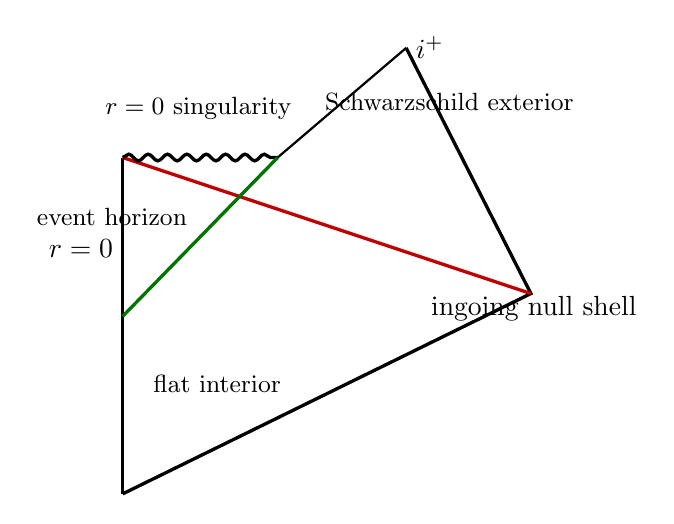
\begin{tikzpicture}[scale=0.96]
\coordinate (A) at (0,-2.8);
\coordinate (B) at (0,1.65);
\coordinate (C) at (2.05,1.65);
\coordinate (D) at (5.4,-0.15);
\coordinate (E) at (3.75,3.10);
\coordinate (H0) at (0,-0.45);
\draw[very thick] (A)--(B);
\draw[very thick] (A)--(D)--(E);
\draw[very thick,red!75!black] (D)--(B);
\draw[very thick,decorate,decoration={snake,amplitude=1.2pt,segment length=7pt}] (B)--(C);
\draw[very thick,green!45!black] (H0)--(C);
\draw[thick] (C)--(E);
\node[left] at (0,0.45) {\(r=0\)};
\node[below right] at (3.95,-0.05) {ingoing null shell};
\node[font=\small] at (1.25,-1.35) {flat interior};
\node[font=\small,anchor=west] at (2.55,2.38) {Schwarzschild exterior};
\node[above,font=\small] at (1.0,2.02) {\(r=0\) singularity};
\node[above left,font=\small] at (0.98,0.62) {event horizon};
\node[right] at (E) {\(i^+\)};
\end{tikzpicture}
\caption{붕괴 기하. 빨간 껍질이 평탄한 내부와 슈바르츠실트 외부를 잇습니다. 초록색 사건의 지평선은 평탄 영역에서 더 이른 시점에 시작해 블랙홀 영역의 미래 경계에서 끝납니다.}
\label{fig:l05-collapse}
\end{figure}

이 구성은 영원한 해에서 남았던 질문에 답합니다. 붕괴로 만들어진 블랙홀에는 과거 화이트홀도 두 번째 점근 우주도 없습니다. 하지만 미래 특이점은 여전히 있습니다.

\section{지평선은 전역적 경계다}

정지 슈바르츠실트 기하에서 지평선을 나타내던 옛 표기 \(r=2GM\)는 동역학적 시공간에서 필요한 정의가 아닙니다.

\begin{definition}
미래 사건의 지평선은 미래지향 인과 신호를 미래 영무한대까지 보낼 수 있는 사건들의 집합을 둘러싼 경계입니다.
\end{definition}

붕괴 도표에서 탈출에 간신히 실패하는 바깥쪽 영선을 따라가 보십시오. 그 바로 바깥쪽의 빛살은 무한대에 도달하고, 바로 안쪽의 빛살은 특이점에서 끝납니다. 그 둘을 가르는 선이 실제 지평선입니다.

\begin{figure}[htbp]
\centering
\includegraphics[width=0.72\textwidth]{lecture_05_figure_06.png}
\caption{칠판의 구성이 완성된 모습. 유입 껍질은 빨간색이고 사건의 지평선은 초록색입니다. 초록색 선의 일부는 껍질 아래쪽의 아직 평탄한 영역에 놓여 있습니다.}
\lectureframe{00:39:10.000}
\end{figure}

이제 놀라운 특징을 피할 수 없습니다. 지평선은 껍질이 아직 도달하지 않은 영역까지 과거 방향으로 뻗어 있습니다. 그곳의 기하는 국소적으로 평탄하며, 그 선을 지나는 관측자는 곡률의 파동이나 벽, 섬광을 감지하지 못합니다. 그런데도 관측자는 이미 무한대에 도달할 수 없습니다. 미래의 껍질이 가능한 모든 탈출 경로를 닫을 것이기 때문입니다. 사건의 지평선은 바로 이런 전역적 의미에서 목적론적입니다. 지평선을 찾으려면 시공간의 미래 전체를 알아야 합니다.\editorialnote{매끄러운 사건의 지평선을 막 통과했는지 국소 실험으로 알아낼 수는 없습니다. 겉보기 지평선이나 포획 지평선처럼 더 국소적인 다른 개념도 있으며, 붕괴 중에는 사건의 지평선과 일치하지 않을 수 있습니다.}

배수구 비유는 인과관계의 핵심을 드러냅니다. 고요한 호수에서 막힌 배수구 근처에 있는 노 젓는 사람을 생각해 보십시오. 마개가 영원히 그대로라면 노 젓는 사람은 떠날 수 있습니다. 누군가 반드시 마개를 뽑으리라는 것을 안다면, 아직 물이 흐르지 않아도 나중에 생길 물살 때문에 탈출이 불가능해질 수 있습니다. 얼어붙은 나이아가라 폭포도 같은 점을 보여 줍니다. 물이 잔잔하다고 해서 앞으로 안전한 경로가 보장되는 것은 아닙니다.

\begin{classroomqa}
\audiencequestion{빛의 구형 껍질이 점점 더 집중되기 때문에 마개가 뽑히는 건가요?\lecturetimestamp{00:43:13}}
\lecturerresponse{집중으로 블랙홀이 만들어지지만, 여기서 배수구 이야기는 더 좁은 목적에 쓰입니다. 국소적으로 극적인 일이 일어나기 전에도 이미 돌아올 수 없는 경계를 넘어섰을 수 있다는 점을 설명합니다.}
\end{classroomqa}

\subsection{커지는 구면으로 이루어진 지평선}

축약된 지평선의 각 점은 \(S^2\)를 나타냅니다. 지평선의 시작점에서 그 구면의 넓이는 0입니다. 지평선을 따라 위쪽으로 가면 구면이 커져 면적 반지름이
\begin{equation}
R_s=\frac{2GM}{c^2}.
\end{equation}
에 도달합니다. 정지한 블랙홀에서는 그 크기를 유지하고, 에너지가 더 유입되면 다시 커집니다.

\editorialnote{이상화한 구형 붕괴 도표에서 지평선의 생성선들은 \(r=0\) 위의 형성점, 즉 주름점에서 만납니다. 넓이가 0인 것은 이 극한의 구면입니다. 이 진술을 유한한 슈바르츠실트 지평선이 갑자기 한 점으로 쪼그라든다는 뜻으로 읽어서는 안 됩니다.}

\subsection{먼 거리 관측자가 재구성할 수 있는 것}

이어지는 긴 논의에서는 전역적 지평선 안에 이미 들어간 관측자와 그 관측자가 그곳에 이르게 된 과정을 구분합니다.

\begin{classroomqa}
\audiencequestion{껍질이 도달하기 전에 갇힌 사람은 어떤 상태인가요? 먼 거리 관측자의 관점에서는 지평선 바깥에 있나요?\lecturetimestamp{00:44:03}}
\lecturerresponse{아닙니다. 세계선이 사건의 지평선 안쪽에 놓이면 그 미래는 특이점에 이르고, 그곳에서 새로운 신호가 먼 거리 관측자에게 도달하지 않습니다. 하지만 그 사람이 그곳에서 존재하기 시작한 것은 아닙니다. 앞서 그 사람을 이루던 입자나 조상, 또는 그 밖의 선행 에너지는 관측 가능한 영역에서 들어왔습니다.}
\end{classroomqa}

따라서 먼 거리 관측자는 선행 물질이 지평선에 접근하는 것을 볼 수 있지만, 지평선 너머에서 오는 신호는 받지 못합니다. 유입 껍질 너머를 보는 데 모순은 없습니다. 껍질은 빛으로 이루어져 있고, 관측자는 껍질 자체를 볼 수 있으며 블랙홀이 형성되었다고 추론할 수도 있습니다.

\begin{classroomqa}
\audiencequestion{시선이 붕괴하는 껍질을 통과하나요? 외부 관측자는 블랙홀이 형성된 사실을 여전히 알 수 있나요?\lecturetimestamp{00:46:51}}
\lecturerresponse{그렇습니다. 관측자는 유입 껍질을 볼 수 있고, 아직 탈출할 수 있는 빛이 껍질을 가로지르는 경로를 따라 올 때 그 빛을 받을 수도 있습니다. 이상하게 보이는 점은 껍질이 중심에 도달하기도 전에 선행 물질이 새로 정해진 지평선에 접근한다는 것입니다.}
\end{classroomqa}

\begin{classroomqa}
\audiencequestion{이것도 외부에서 보면 물질이 지평선에 압축되어 있는 듯 보인다는 규칙의 연장인가요?\lecturetimestamp{00:47:49}}
\lecturerresponse{그렇습니다. 외부 관점의 기술에서는 물질이 지평선에 계속 붙어 있는 듯 보이고, 적색편이는 점점 커집니다. 이후 블랙홀이 양자 과정으로 증발하면서 상황이 달라집니다.}
\end{classroomqa}

이 외부 관점의 기술은 다음 주제로 이어집니다. 정보가 2차원 표면에 붙어 있는 듯 보인다면, 블랙홀 엔트로피가 그 표면의 넓이에 비례한다는 사실도 덜 놀랍습니다.

\section{엔트로피와 무한대에서 관측되는 온도}

큰 지평선 근처에서는 작은 실험실에서 평면 지구 근사를 쓰듯, 구면을 국소 평면으로 바꿔 생각할 수 있습니다. 그러면 앞서 살펴본 두 가지 사실을 함께 놓을 수 있습니다:
\begin{equation}
\begin{aligned}
S_{\mathrm{BH}}&\propto A_H,\\
\Delta A_H&\sim \ell_P^2
\quad\text{per added bit, schematically}.
\end{aligned}
\end{equation}
플랑크 면적당 1비트라는 기억법은 면적 법칙을 나타낼 뿐, 미시적 유도는 아닙니다.

슈바르츠실트 블랙홀에서 멀리 떨어진 곳에서 측정한 호킹 온도는
\begin{equation}
T_H=\frac{\hbar c^3}{8\pi GMk_B}.
\label{eq:l05-hawking}
\end{equation}
입니다. \(R_s=2GM/c^2\)을 사용하면
\begin{equation}
T_H=\frac{\hbar c}{4\pi k_B R_s}.
\label{eq:l05-hawking-radius}
\end{equation}
을 얻습니다.
따라서 큰 블랙홀일수록 차갑습니다.

\begin{classroomqa}
\audiencequestion{온도는 위치에 따라 달라질 수 있나요?\lecturetimestamp{00:52:43}}
\lecturerresponse{일상 대화에서는 당연히 그럴 수 있습니다. 뉴욕과 스탠퍼드의 온도가 같을 필요는 없습니다. 더 정확한 질문은 중력 열평형 상태에 있는 계에 관한 것입니다. 그런 계에서는 적색편이된 평형 온도는 일정하더라도 국소 온도계의 눈금은 높이에 따라 달라질 수 있습니다.}
\end{classroomqa}

온도는 국소적인 운동 에너지로 측정합니다. 가열된 지구 위의 희박한 대기에서 분자는 올라가면서 운동 에너지를 잃고 내려오면서 얻습니다. 광자는 위쪽으로 갈 때 적색편이되고 아래쪽으로 갈 때 청색편이됩니다. 따라서 낮은 곳의 온도계와 높은 곳의 온도계가 같은 국소 에너지 척도를 가리킬 필요는 없습니다.

정적인 시공간에서 평형 관계는
\begin{equation}
T_{\mathrm{loc}}(r)\sqrt{-g_{tt}(r)}=T_\infty,
\label{eq:l05-tolman}
\end{equation}
이며, 이를 톨먼 법칙이라고 합니다. 식~\eqref{eq:l05-hawking}의 호킹 온도는 \(T_\infty\), 즉 무한대에서 정규화한 온도계 눈금입니다.

\section{지평선 근처의 뜨거운 정지 대기}

\(\rho\)를 지평선에서 바깥쪽으로 잰 고유 거리라고 합시다. 큰 슈바르츠실트 지평선 가까이에서는 식~\eqref{eq:l05-tolman}가
\begin{equation}
k_B T_{\mathrm{loc}}(\rho)
\simeq\frac{\hbar c}{2\pi\rho},
\label{eq:l05-local-temperature-si}
\end{equation}
가 되며, 단위계 \(c=\hbar=k_B=1\)에서는
\begin{equation}
T_{\mathrm{loc}}(\rho)=\frac{1}{2\pi\rho}.
\label{eq:l05-local-temperature}
\end{equation}

\begin{figure}[htbp]
\centering
\includegraphics[width=0.72\textwidth]{lecture_05_figure_07.png}
\caption{칠판에 표시한 무한대의 호킹 온도와 지평선 근처의 국소 온도 \(T(\rho)=1/(2\pi\rho)\).}
\lectureframe{01:02:40.000}
\end{figure}

케이블에 고정해 매단 작은 온도계는 고정된 \(\rho\)에서 아래로 내릴수록 온도가 올라간다고 측정합니다. 정지한 그 열적 대기에 놓인 원자는 들뜬 다음 이온화되고, 이어서 해리됩니다. 국소 에너지가 더 커지면 원자핵과 강입자마저 온전한 상태를 유지하지 못합니다. 사람을 발부터 내리면 기억에 남을 만한 진단이 나옵니다. 발이 뜨겁습니다.

\emph{매달아} 두었다는 표현이 중요합니다. 이 발산은 가속으로 정지 상태를 유지하는 검출기에 해당합니다. 이는 외부 시간에 대해 적색편이된 열적 대기를 설명합니다. 자유 낙하 검출기는 다른 궤적을 따르며, 충분히 큰 블랙홀의 규칙적인 양자 상태에서는 지평선에서 발산하는 열적 대기를 겪지 않을 수 있습니다.\editorialnote{이 구분은 정지 관측자가 보는 톨먼 온도와 가속 온도를 자유 낙하 관측자의 규칙적인 국소 경험과 구별합니다. 강의에서는 용어만으로 이 대조를 해소하지 않고, 의도적으로 조작 가능한 수수께끼로 제시합니다.}

이온화 문턱은 이 충돌을 구체적으로 보여 줍니다.

\begin{classroomqa}
\audiencequestion{수소를 이온화하는 데 필요한 에너지는 얼마인가요?\lecturetimestamp{01:06:53}}
\lecturerresponse{수업에서는 \(13\)전자볼트라고 답해 \(13.6\,\mathrm{eV}\) 바닥상태 이온화 에너지를 정확히 짚었습니다. 이에 덧붙인 수천 켈빈이라는 추정값은 너무 낮지만, 이 논증에는 유한한 문턱값이 있다는 사실만 필요합니다.}
\end{classroomqa}

실제로,
\begin{equation}
\frac{13.6\,\mathrm{eV}}{k_B}\simeq1.58\times10^5\,\mathrm{K}.
\end{equation}
정지 온도가 이온화 규모에 도달하는 작은 고유 거리 \(\rho_{\mathrm{ion}}\)가 존재합니다. 정지 관측자 관점의 외삽에 따르면 원자는 지평선 바깥인 그 지점에서 이미 이온화되어 있어야 합니다. 반면 자유 낙하하는 원자는 국소적인 벽을 겪지 않으며 유한한 고유 시간 안에 지평선을 통과할 수 있다고 예상합니다. 외부 관측자는 이 두 기술 가운데 어느 쪽이 맞는지 판별하는 실험을 할 수 있을까요?

\section{하이젠베르크 현미경}

블랙홀에 이 질문을 적용하기에 앞서 광자 현미경을 떠올려 봅시다. 입자의 위치를 \(\Delta x\)의 분해능으로 알아내려면 탐침의 파장은
\begin{equation}
\lambda\lesssim\Delta x.
\end{equation}
을 만족해야 합니다.
그러면 광자 하나는 적어도 다음 운동량을 갖습니다.
\begin{equation}
p_\gamma\gtrsim\frac{\hbar}{\Delta x}.
\label{eq:l05-microscope}
\end{equation}
그 광자를 산란시키면 같은 규모의 반동이 생깁니다. 먼저 위치를 측정하고 곧바로 속도를 확인하면, 두 번째 측정은 첫 번째 측정으로 바뀐 상태를 봅니다. 실험이 바로 배제하려던 조건을 만들어 내는 셈입니다.

\begin{figure}[htbp]
\centering
\includegraphics[width=0.70\textwidth]{lecture_05_figure_08.png}
\caption{현미경으로 \(\Delta x\gtrsim\lambda\)과 \(p_\gamma\gtrsim\hbar/\Delta x\)을 추정합니다.}
\lectureframe{01:11:50.000}
\end{figure}

이것은 단순히 고전 광학의 한계가 아닙니다. 고전파의 세기는 얼마든지 약하게 만들 수 있지만, 양자역학에서는 검출이 성공하려면 적어도 양자 하나가 필요합니다. 따라서 공간 분해능을 높이려면 유한한 운동량 전달이 불가피합니다.

\section{지평선 근처 실험}

이제 \(\rho_{\mathrm{ion}}\)에서 시작되는 층을 원자가 낙하한다고 합시다. 정지 좌표계에 대해서 원자는 안쪽으로 거의 \(c\)의 속도로 움직이므로, 지평선을 통과하기 전까지 남은 시간 간격은 대략
\begin{equation}
\Delta\tau\sim\frac{\rho_{\mathrm{ion}}}{c}.
\label{eq:l05-fall-time}
\end{equation}
입니다.
지평선을 통과한 뒤에는 어떤 결과도 외부로 보낼 수 없습니다. 이 짧은 시간 동안 원자가 온전한 상태인지 이온화되었는지 판별해야 합니다.

그 층 안에서 원자를 분해해 보려면
\begin{equation}
\lambda\lesssim\rho_{\mathrm{ion}}.
\end{equation}
이어야 합니다.
따라서 탐침 에너지에는 다음 조건이 따릅니다.
\begin{equation}
E_\gamma=cp_\gamma
\gtrsim\frac{\hbar c}{\rho_{\mathrm{ion}}}.
\label{eq:l05-probe-energy}
\end{equation}
계수 \(2\pi\)를 제외하면 이는 식~\eqref{eq:l05-local-temperature-si}와 같은 규모입니다:
\begin{equation}
E_\gamma\gtrsim2\pi k_B T_{\mathrm{loc}}(\rho_{\mathrm{ion}}).
\label{eq:l05-probe-temperature}
\end{equation}
사건을 분해해 볼 만큼 에너지가 큰 광자는 원자를 이온화할 만큼도 에너지가 큽니다.

\begin{figure}[htbp]
\centering
\includegraphics[width=0.72\textwidth]{lecture_05_figure_09.png}
\caption{칠판의 지평선 근처 추정: \(\lambda<\rho\)이면 국소 탐침 에너지가 \(\hbar c/\rho\) 규모여야 합니다.}
\lectureframe{01:18:30.000}
\end{figure}

\begin{classroomqa}
\audiencequestion{그 고에너지 광자는 자유 낙하 좌표계에서도 원자를 이온화하나요?\lecturetimestamp{01:19:07}}
\lecturerresponse{그렇습니다. 실제로 에너지가 큰 양자가 원자에 부딪히며, 원자의 국소 좌표계에서도 반동이나 이온화가 일어납니다. 이 측정은 방해받지 않은 낙하를 알아내지 않습니다. 방해받은 낙하로 바꿉니다.}
\end{classroomqa}

\begin{classroomqa}
\audiencequestion{원자가 실험 없이 그저 낙하하면 어떻게 되나요?\lecturetimestamp{01:19:39}}
\lecturerresponse{그렇다면 이 특정한 교란은 없습니다. 외부 관측자가 고분해능 실험을 수행한다면 원자는 곤란한 상황에 처합니다. 이 논증은 측정하지 않은 낙하자가 타버린다는 증명이 아니라, 외부에서 무엇을 검증할 수 있는지에 관한 것입니다.}
\end{classroomqa}

\subsection{온도계나 송신기로는 더 잘 측정할 수 없나요?}

장치를 옮겨도 정보 문제는 사라지지 않습니다.

\begin{classroomqa}
\audiencequestion{더 멀리서 측정해 기울기를 추론하거나, 자유 낙하 온도계가 온도를 기록하게 한 다음 나중에 그 기록을 회수할 수는 없나요?\lecturetimestamp{01:19:51}}
\lecturerresponse{지평선 근처의 기록을 알아내려면 무언가가 온도계와 상호작용하고 양자를 통해 정보를 되돌려 보내야 합니다. 온도계의 방향을 돌리려면 격렬한 가속이 필요하고, 원격으로 읽으려면 방출이나 산란이 필요합니다. 어느 방법이든 방해받지 않은 이력을 확인하려던 물리적 계를 변화시킵니다.}
\end{classroomqa}

\begin{classroomqa}
\audiencequestion{작은 공간 분해능에 필요한 높은 탐침 에너지와, 반사된 관측 신호를 지평선 근처 영역 밖으로 가져오는 문제는 같은 어려움인가요?\lecturetimestamp{01:21:51}}
\lecturerresponse{둘은 적색편이로 연결된 같은 에너지 규모의 양면입니다. 광자가 밖으로 올라오면서 에너지를 잃으므로 무한대에 도달할 때는 에너지가 낮을 수 있지만, 원자를 분해해 볼 때는 국소 진동수가 높아야 합니다.}
\end{classroomqa}

\editorialnote{지평선 바로 바깥에서 방출된 광자도 탈출하려면 반드시 높은 에너지를 가져야 하는 것은 아닙니다. 여기서 결정적인 조건은 고유 시간과 거리가 \(\rho\) 규모인 동안 일어난 사건을 광자가 담아야 한다는 점입니다. 중력 적색편이는 이 높은 국소 진동수를 훨씬 낮은 점근 진동수와 연결합니다.}

\begin{classroomqa}
\audiencequestion{외부 광자에 맞지 않고 물체가 스스로 정보를 방출할 수는 없나요?\lecturetimestamp{01:22:51}}
\lecturerresponse{가능합니다. 하지만 국소 방출도 짧은 시간 동안 무슨 일이 일어났는지 식별하는 데 필요한 대역폭을 가져야 합니다. 방출은 물체에 반동도 줍니다. 반사광을 송신기로 바꾸어도 아무런 대가 없이 기록을 얻을 수는 없습니다.}
\end{classroomqa}

\begin{classroomqa}
\audiencequestion{낙하하는 원자는 선호되는 방향을 갖습니다. 그 방향성을 가진 운동 에너지를 온도라고 부르는 건가요?\lecturetimestamp{01:23:10}}
\lecturerresponse{아닙니다. 야구공을 던진다고 해서 공이 뜨거워지는 것은 아닙니다. 물체의 집단적 낙하 에너지와 열적 요동은 서로 다릅니다. 이 논증에서 말하는 온도는 주위의 정적 복사 대기에 해당하며, 원자의 질량중심 운동에 해당하는 것이 아닙니다.}
\end{classroomqa}

\begin{classroomqa}
\audiencequestion{함께 낙하하는 실험실에서 자기장을 이용해 원자가 이온화되었는지 확인할 수 있나요?\lecturetimestamp{01:23:50}}
\lecturerresponse{실험실 안에서 국소적인 측정을 할 수는 있습니다. 문제는 지평선을 넘기 전에 그 결과를 바깥으로 전달하는 일입니다. 그러려면 다시 상호작용이 필요하고, 필요한 국소 분해능을 갖춘 출사 양자도 필요합니다.}
\end{classroomqa}

\begin{classroomqa}
\audiencequestion{온도계에 송신기를 내장하면 장치를 망가뜨릴 정도로 큰 국소 에너지가 필요할까요?\lecturetimestamp{01:24:57}}
\lecturerresponse{그것은 같은 장애물을 공학적 관점에서 표현한 것입니다. 지평선에 충분히 가까워지면, 관련된 국소 규모에서 신호에 필요한 에너지는 측정하려는 열적 규모와 비슷해집니다.}
\end{classroomqa}

\begin{classroomqa}
\audiencequestion{고온 영역이 너무 얇아서 여유 있게 측정할 시간이 없나요?\lecturetimestamp{01:25:15}}
\lecturerresponse{그렇습니다. 그 고유 두께는 \(\rho\) 정도이고, 통과 시간은 \(\rho/c\) 정도입니다. 이 한계를 공간 분해능으로 표현할 수도 있고 시간 대역폭으로 표현할 수도 있습니다. 어느 쪽으로 표현하든 큰 국소 운동량이나 에너지가 필요합니다.}
\end{classroomqa}

이에 대응하는 시간·대역폭 추정은 다음과 같습니다.
\begin{equation}
\Delta E\,\Delta\tau\gtrsim\hbar.
\end{equation}
여기서는 이를 \(\Delta x\,\Delta p\geq\hbar/2\)와 지위가 같은 연산자 불확정성 관계가 아니라, 푸리에 분석에 따른 분해능 또는 조작적 분해능의 한계로 읽어야 합니다. 강의에서는 시간·에너지 불확정성 관계를 휴리스틱하게 사용합니다. 공간 분해능에서 유도한 식~\eqref{eq:l05-probe-energy}이 논증에서 더 확고한 부분입니다.

\begin{classroomqa}
\audiencequestion{에너지가 낮고 분해능이 낮은 탐침을 많은 원자에 사용한 뒤 통계적으로 답을 알아낼 수는 없나요?\lecturetimestamp{01:26:26}}
\lecturerresponse{타당한 질문이며, 강의실에서는 답을 열어 둡니다. 원자 하나는 단 한 번만 통과하고, 신호를 알아내더라도 지평선 부근에서 짧게 일어난 사건을 식별할 만큼 충분한 정보를 담아야 합니다. 강의에서는 불확정성 원리를 근거로 들지만, 통계적 방법이 불가능하다는 완전한 증명은 제시하지 않습니다.}
\end{classroomqa}

\enlargethispage{2\baselineskip}
\section{확립된 것과 확립되지 않은 것}

이 논증은 자유 낙하하는 사람이 발산하는 정적 온도를 반드시 느낀다고 예측하지 않습니다.

\begin{classroomqa}
\audiencequestion{낙하하는 사람이 그 온도를 느끼지 않을 것이라고 예측할 수 있다는 말인가요?\lecturetimestamp{01:27:38}}
\lecturerresponse{아닙니다. 결론은 더 제한적입니다. 원자가 고온 교란을 겪지 않았음을 확인하려고 설계한 외부 실험은 그와 같은 규모의 교란을 일으킵니다. 이 조작적 분석으로 확립되는 것은 그뿐입니다.}
\end{classroomqa}

따라서 이 결론은 방화벽 정리가 아니며, 낙하자가 화상을 입는다는 증명도, 아무 일도 일어나지 않는다는 증명도 아닙니다. 이는 외부에서 확인할 수 있는 범위의 한계입니다. \emph{교란되지 않은 지평선 부근 사건을 분해하려면 그 사건을 교란하는 탐침이 필요합니다}.
실험을 수행하면 그 양자들이 실험이 검증하려 했던 효과를 일으킵니다. 실험을 수행하지 않는다면, 이 논증만으로는 실험적으로 접근 가능한 사실이 더해지지 않습니다. 이중 슬릿 실험과의 비교는 의도적입니다. 경로를 측정하지 않고 어느 슬릿을 통과했는지 묻는 것과 상호작용 없이 외부 장치가 무엇을 확인해 주는지 묻는 것은 모두, 제안된 증거로는 얻을 수 없는 조작적 답을 붙이려는 시도입니다.
